\section{Il bilancio di esercizio}
\begin{figure}[H]
    \centering
    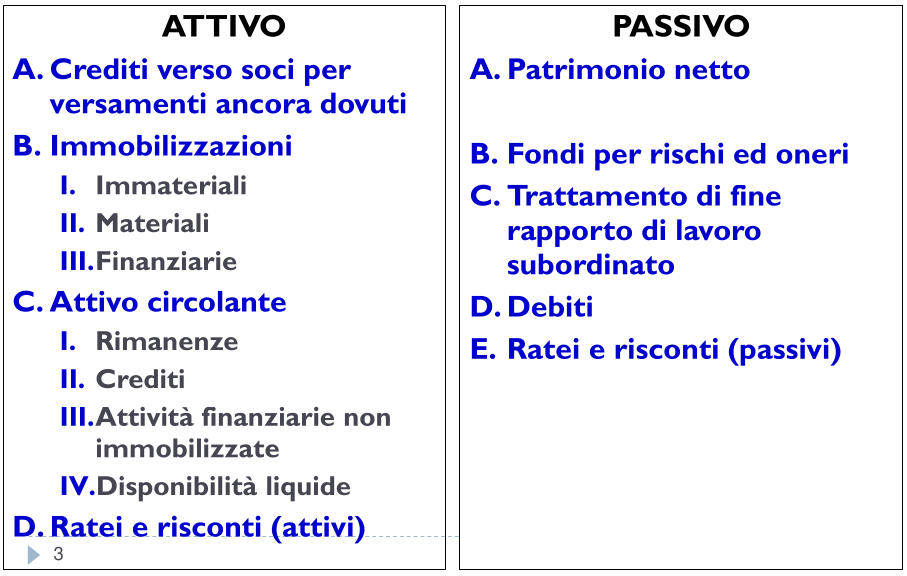
\includegraphics[width=0.7\linewidth]{2/img/Screenshot from 2022-07-06 22-20-49.png}
\end{figure}
\subsection{Stato patrimoniale: Attività}


\subsubsection{Crediti verso soci per versamenti ancora dovuti}

è 0 se il capitale sociale è stato versato dai soci.

\subsubsection{Immobilizazzione}
Immobilizzazioni immateriali:
\begin{itemize}
    \item costi di impianto e di ampliamento
    \item costi di sviluppo
    \item diritto di brevetto
    \item concessioni, licenze, marchi e diritti simili
    \item avviamento
    \item immobilizzazi in corso e acconti
    \item altre
\end{itemize}

Immobilizzazioni materiali:
\begin{itemize}
    \item terreni e fabbricati
    \item impianti e macchinari
    \item attrezzature
    \item altri begin
    \item Immobilizazzione in  corso e acconti
\end{itemize}


Immobilizzazioni finanziarie:
\begin{itemize}
    \item partecipazioni in imprese
    \item Creditialtri titoli
    \item strumenti finanziari derivati attivi
\end{itemize}

\subsubsection{Attivo circolare}
rimanenze:
\begin{itemize}
    \item materie prime ecc
    \item prodotti in corso di lavorazione
    \item lavori in corso
    \item prodotti finiti e merci
    \item acconti
\end{itemize}

crediti:
\begin{itemize}
    \item verso cliente
    \item verso imprese controllate
    \item verso imprese collegate
    \item verso imprese controllanti
    \item crediti tributari
    \item imposte anticipate
\end{itemize}

Attività finanziarie che non costituiscono immobilizzazioni:
\begin{itemize}
    \item patecipazione non strategica in aziende
    \item altre partecipazioni
    \item strumenti derivati attivi
\end{itemize}

Disponibilità liquide:
\begin{itemize}
    \item depositi bancari e postali
    \item assegni
    \item denaro e valori in cassa
\end{itemize}


\subsubsection{Ratei e riscontri(attivi)}
I ratei attivi rilevano quote di ricavi di competenza dell'esericzio in corso
esigibili nell'esercizio successivo.

I riscontri attivi rettificano quote di costo già rilevate ma di competenza di esercizi passati.


\subsection{Stato patrimoniale: Passività}
\subsubsection{Patrimonio netto}
Insieme delle fonti di capitale proprio(di rischio)
\begin{itemize}
    \item capitale
    \item risetva da sovrapprezzo delle azioni
    \item riserva di rivalutazione
    \item riserva legale
    \item utili(perdite) portati a nuovo
    \item itili(perdita) dell'esercizio
    \item riserva negativa per azioni prorpie in portafoglio 
\end{itemize}

\subsubsection{Fonti per rischi ed oneri}

Soldi da parte per:
\begin{itemize}
    \item quiescenze e robe simili
    \item imposte
    \item strumenti finanziari derivati Passività
    \item altro
\end{itemize}

\subsubsection{TFR dei lavoratori}
accantonamento dei soldi maturati dal dipendente dati via al momento del licenziamento.

\subsubsection{Debiti}
\begin{itemize}
    \item obbligazioni
    \item debiti verso qualcuno
    \item acconti
\end{itemize}

\subsubsection{Ratei e riscontri(passivi)}
I ratei passivi rilevano i quote di costi di competenza dell'esercizio esigibili nell'esercizio successivo.

I risconti passivi rettificano quote di ricavo già rilevate ma
di competenza dell'esercizio successivo.


\subsection{Il conto economico}
\begin{figure}[H]
    \centering
    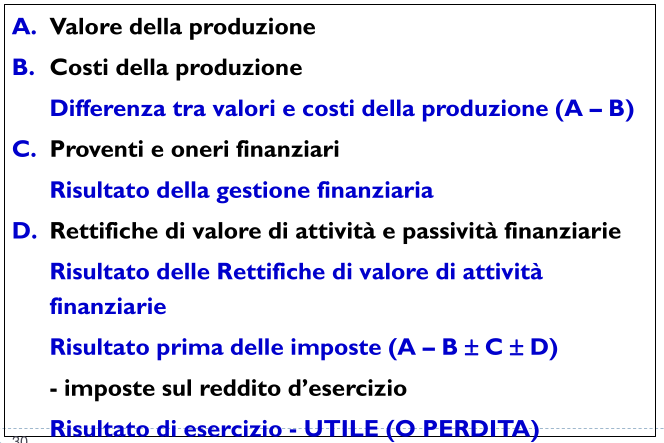
\includegraphics[width=0.7\linewidth]{2/img/Screenshot from 2022-07-07 16-11-55.png}
\end{figure}

\subsubsection{Valore della produzione}
valore di tutti i beni prodotti dall'impresa nell'esercizio
\begin{itemize}
    \item ricavi dalle vendite e delle prestazioni
    \item variazioni delle rimanenze di prodotti in lavorazione
    \item variazioni dei lavori in corso su ordinazione
    \item incremento di immobilizzazione per lavori interni
    \item altri ricavi e proventi
\end{itemize}

\subsubsection{Costi della produzione}
insieme dei costi sostenuti dall'impresa, derivanti sia da attività di
vera e propria trasformazione, sia da attività di supporto.


\begin{itemize}
    \item materie prime
    \item servizi
    \item personale(salari ecc)
    \item ammortamentie svalutazioni
    \item variazione delle rimanenze di magazzino
    \item accantonamento rischi
    \item oneri diversi di gestione
\end{itemize}

\subsubsection{Differenza tra valori e costi della produzione}
MON = margine operativo netto, è il risultato dell'attività operativa dell'impresa.


VAL = valore aggiunto lordo, misura quanto la gestione operativa dell'impresa ha aumentato il valore degli acquisti.

\subsubsection{Proventi e oneri finanziari}
\begin{itemize}
    \item proventi da partecipazioni
    \item interessi e altri oneri
    \item utili e perdite su scambi
\end{itemize}

\subsubsection{Rettifiche di valore di attività e passività finanziarie}
\begin{itemize}
    \item rivalutazione di partecipazioni
    \item svalutazione di partecipazioni
\end{itemize}

\textbf{Risultato prima delle imposte (A - B $\pm$ C $\pm$ D)}